The part of the created system that is described in this chapter is devoted to explaining the main flow of procedures that are required to perform semantic image segmentation with use of Conditional Random Fields. It is presented on a simple example of performing a classification on detected objects in an image basing only on colours of those objects, without incorporating any contextual data. This part of the system was aimed to proof that that with use of Conditional Random Fields it is possible to perform semantic  segmentation of images, which can also contain noised data. The theory behind all the algorithms that were used to accomplish this task has already been presented in \textit{Chapter \ref{chapter:structured_prediction}: \nameref{chapter:structured_prediction}}.

\subsection{System components}

The created system incorporates all the standard components needed for supervised machine learning. To perform semantic image segmentation a dataset of images is needed, that will be described in details in the next section. Images used in the thesis were artificially generated, therefore, the first component of the system is an image generator. Next step is a preprocessing phase, which is fully described in \textit{section \ref{sec:linear_preprocessing}: \nameref{sec:linear_preprocessing}}. Its main goal is to perform a division into superpixels, which limits the complexity of other processes. Having the dataset prepared there is a need to provide a method of transforming data from superpixels into meaningful features that are understandable by the algorithms used in the system. Hence, the next component performs feature extraction with feature selection being done manually. As it has already been presented in the theoretical part, Conditional Random Fields are best modelled with the use of factor graphs, thus the next component performs factorisation. These are all the required steps that are needed to provide input data for two main processes in the created semantic segmentation system which are parameter training and inference. Both of these processes were explained in details in the previous chapter. In a training phase optimal parameters of the created model are learned in a supervised manner with the use of Stochastic Gradient Descent algorithm. For the sake of better visualisation, figure \ref{fig:training_chart_linear} is provided, which shows the main task of each component of the system that is required to obtain a learned model. 
\begin{figure}[ht]
    \centering
    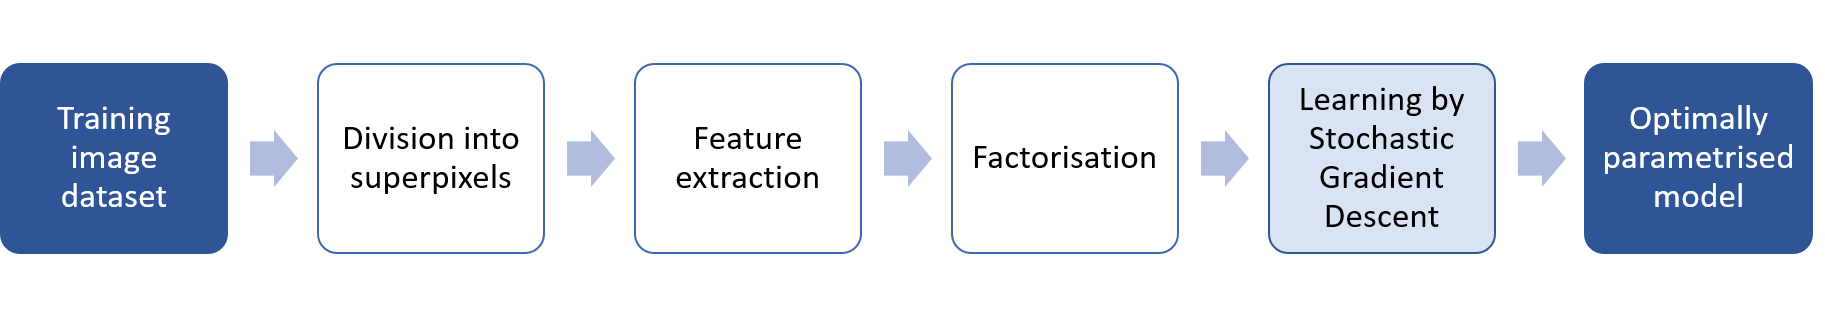
\includegraphics[width=\textwidth]{system_overview/training_chart_linear.png}
    \caption{Workflow required to obtain a trained parametrised model used for semantic image segmentation}
     \label{fig:training_chart_linear}
\end{figure}
Having a properly parametrised model it is possible to perform semantic image segmentation on an unknown image in the next component that conducts a process of maximum a posteriori inference. As it has been explained in the theoretical section, for Conditional Random Fields the most suitable inference algorithm is Loopy Belief propagation. Beliefs are passed along a factor graph model that was constructed for a given test image in a way described by the Min-Sum algorithm. In this component, the most probable configuration of superpixel labels for a given image is found and therefore the task of semantic segmentation is completed. Figure \ref{fig:segmentation_chart_linear} visualises the components that perform tasks required for performing semantic image segmentation with already trained model.
\begin{figure}[ht]
    \centering
    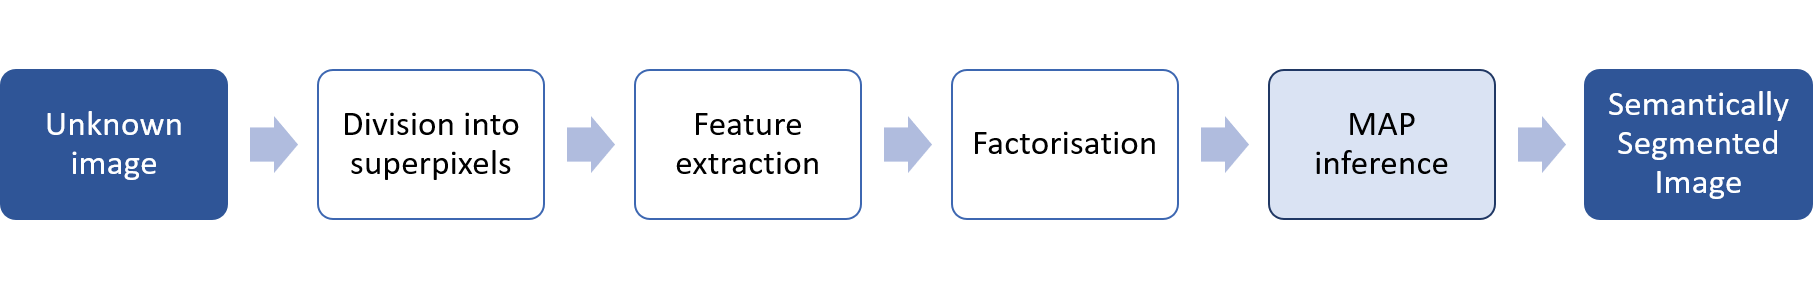
\includegraphics[width=\textwidth]{system_overview/segmentation_chart_linear.png}
    \caption{Workflow required to perform a semantic image segmentation}
     \label{fig:segmentation_chart_linear}
\end{figure}

\subsection{Technological stack}
From all the presented components only the preprocessing stage was implemented with the use of an external library, which was delivered by the supervisor of this thesis. Other components were written from scratch only with the use of some basic Java libraries that facilitate coding and testing such as Apache Commons, log4j or JUnit. As the preprocessing component was incorporated to the system after some progress in implementation of other components had already been made, during the initial planning phase there was no restrictions on the programming tools that are to be used. That is why the technological stack was mainly the matter of personal choice. A language chosen for implementation of this system was Java 1.8. It is a well established language that is platform independent. This is a huge advantage in situations in which the same program is to be developed on two different operating systems, or if the development and testing phases happens on different machines. Furthermore, according to TIOBE Programming Community index \cite{tiobe}, which provides data on language popularity, Java is currently the most popular language and it has been in top three for nearly 20 years. It also has a large availability of free tools, including Eclipse IDE, which was used for development of the system presented in this dissertation. 
When it comes to the hardware on which all the phases of the system development took place, it was a personal computer with processor Intel Core i5-5250U with 8GB of RAM and Windows 10 as an operating system.




